\section{stats.h File Reference}
\label{memctrl_2stats_8h}\index{stats.h@{stats.h}}
{\tt \#include \char`\"{}../kernel/component.h\char`\"{}}\par
{\tt \#include \char`\"{}../kernel/simulator.h\char`\"{}}\par
{\tt \#include \char`\"{}../simIris/data\_\-types/impl/irisEvent.h\char`\"{}}\par
{\tt \#include \char`\"{}request.h\char`\"{}}\par


Include dependency graph for memctrl/stats.h:\nopagebreak
\begin{figure}[H]
\begin{center}
\leavevmode
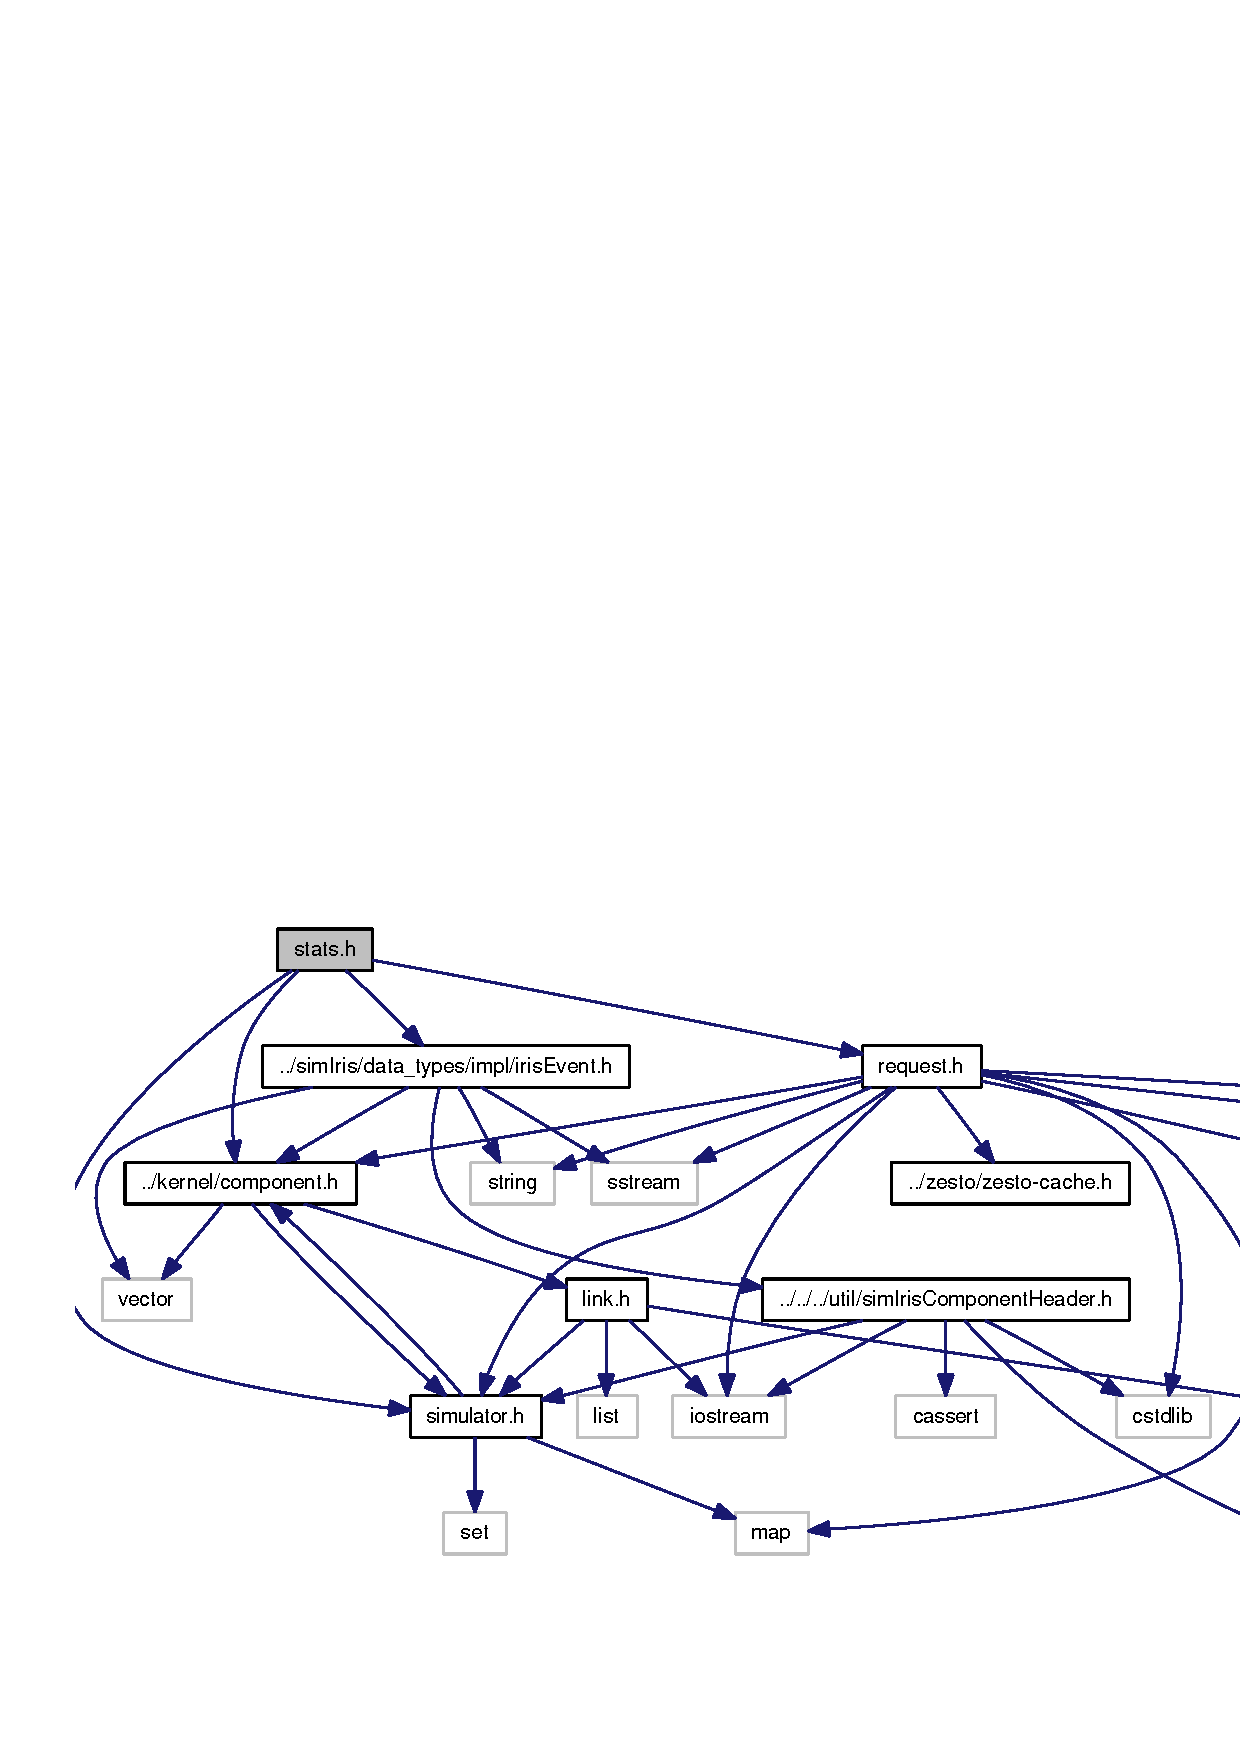
\includegraphics[width=420pt]{memctrl_2stats_8h__incl}
\end{center}
\end{figure}


This graph shows which files directly or indirectly include this file:\nopagebreak
\begin{figure}[H]
\begin{center}
\leavevmode
\includegraphics[width=318pt]{memctrl_2stats_8h__dep__incl}
\end{center}
\end{figure}
\subsection*{Classes}
\begin{CompactItemize}
\item 
class {\bf Statistic}
\item 
class {\bf PowerStats}
\end{CompactItemize}
\subsection*{Defines}
\begin{CompactItemize}
\item 
\#define {\bf MaxVcc}~1.58
\item 
\#define {\bf MinVcc}~1.43
\item 
\#define {\bf DQS}~2
\item 
\#define {\bf IDD0}~120
\item 
\#define {\bf IDD2PS}~10
\item 
\#define {\bf IDD2PF}~25
\item 
\#define {\bf IDD2N}~60
\item 
\#define {\bf IDD3P}~40
\item 
\#define {\bf IDD3N}~65
\item 
\#define {\bf IDD4R}~250
\item 
\#define {\bf IDD4W}~225
\item 
\#define {\bf IDD5A}~260
\item 
\#define {\bf t\_\-CK}~1.25
\item 
\#define {\bf SysVdd}~1.5
\item 
\#define {\bf SysClk}~800
\item 
\#define {\bf BL}~8
\item 
\#define {\bf PdqRD}~5.3
\item 
\#define {\bf PdqWR}~13.2
\item 
\#define {\bf PdqRDoth}~0
\item 
\#define {\bf PdqWRoth}~0
\end{CompactItemize}


\subsection{Define Documentation}
\index{memctrl/stats.h@{memctrl/stats.h}!BL@{BL}}
\index{BL@{BL}!memctrl/stats.h@{memctrl/stats.h}}
\subsubsection[{BL}]{\setlength{\rightskip}{0pt plus 5cm}\#define BL~8}\label{memctrl_2stats_8h_d567ea9864a3046e47ab69cdc050ecfa}




Definition at line 132 of file memctrl/stats.h.

Referenced by PowerStats::CalcPower(), and Statistic::CalculateAggregateStats().\index{memctrl/stats.h@{memctrl/stats.h}!DQS@{DQS}}
\index{DQS@{DQS}!memctrl/stats.h@{memctrl/stats.h}}
\subsubsection[{DQS}]{\setlength{\rightskip}{0pt plus 5cm}\#define DQS~2}\label{memctrl_2stats_8h_2ed01491cb4167104350262d51906b9f}




Definition at line 118 of file memctrl/stats.h.

Referenced by PowerStats::CalcPower().\index{memctrl/stats.h@{memctrl/stats.h}!IDD0@{IDD0}}
\index{IDD0@{IDD0}!memctrl/stats.h@{memctrl/stats.h}}
\subsubsection[{IDD0}]{\setlength{\rightskip}{0pt plus 5cm}\#define IDD0~120}\label{memctrl_2stats_8h_c5d55bab190c738b63e338bad3e3ca3a}




Definition at line 120 of file memctrl/stats.h.

Referenced by PowerStats::CalcPower().\index{memctrl/stats.h@{memctrl/stats.h}!IDD2N@{IDD2N}}
\index{IDD2N@{IDD2N}!memctrl/stats.h@{memctrl/stats.h}}
\subsubsection[{IDD2N}]{\setlength{\rightskip}{0pt plus 5cm}\#define IDD2N~60}\label{memctrl_2stats_8h_a7065efe3389eee833eb071f3bf9bfac}




Definition at line 123 of file memctrl/stats.h.

Referenced by PowerStats::CalcPower().\index{memctrl/stats.h@{memctrl/stats.h}!IDD2PF@{IDD2PF}}
\index{IDD2PF@{IDD2PF}!memctrl/stats.h@{memctrl/stats.h}}
\subsubsection[{IDD2PF}]{\setlength{\rightskip}{0pt plus 5cm}\#define IDD2PF~25}\label{memctrl_2stats_8h_43e6e95c5e875592749eb53405c821d0}




Definition at line 122 of file memctrl/stats.h.

Referenced by PowerStats::CalcPower().\index{memctrl/stats.h@{memctrl/stats.h}!IDD2PS@{IDD2PS}}
\index{IDD2PS@{IDD2PS}!memctrl/stats.h@{memctrl/stats.h}}
\subsubsection[{IDD2PS}]{\setlength{\rightskip}{0pt plus 5cm}\#define IDD2PS~10}\label{memctrl_2stats_8h_726029c62317a151ec1046a2ddc48fcb}




Definition at line 121 of file memctrl/stats.h.\index{memctrl/stats.h@{memctrl/stats.h}!IDD3N@{IDD3N}}
\index{IDD3N@{IDD3N}!memctrl/stats.h@{memctrl/stats.h}}
\subsubsection[{IDD3N}]{\setlength{\rightskip}{0pt plus 5cm}\#define IDD3N~65}\label{memctrl_2stats_8h_308add993bb6cc0b4a85c178f08b7724}




Definition at line 125 of file memctrl/stats.h.

Referenced by PowerStats::CalcPower().\index{memctrl/stats.h@{memctrl/stats.h}!IDD3P@{IDD3P}}
\index{IDD3P@{IDD3P}!memctrl/stats.h@{memctrl/stats.h}}
\subsubsection[{IDD3P}]{\setlength{\rightskip}{0pt plus 5cm}\#define IDD3P~40}\label{memctrl_2stats_8h_a8796a2d6af26cc54ed02cfa473bc940}




Definition at line 124 of file memctrl/stats.h.

Referenced by PowerStats::CalcPower().\index{memctrl/stats.h@{memctrl/stats.h}!IDD4R@{IDD4R}}
\index{IDD4R@{IDD4R}!memctrl/stats.h@{memctrl/stats.h}}
\subsubsection[{IDD4R}]{\setlength{\rightskip}{0pt plus 5cm}\#define IDD4R~250}\label{memctrl_2stats_8h_d5b1fa999b5a43e0dc1936cc15c99972}




Definition at line 126 of file memctrl/stats.h.

Referenced by PowerStats::CalcPower().\index{memctrl/stats.h@{memctrl/stats.h}!IDD4W@{IDD4W}}
\index{IDD4W@{IDD4W}!memctrl/stats.h@{memctrl/stats.h}}
\subsubsection[{IDD4W}]{\setlength{\rightskip}{0pt plus 5cm}\#define IDD4W~225}\label{memctrl_2stats_8h_752ac0260f3befd9243fab14a7ff0994}




Definition at line 127 of file memctrl/stats.h.

Referenced by PowerStats::CalcPower().\index{memctrl/stats.h@{memctrl/stats.h}!IDD5A@{IDD5A}}
\index{IDD5A@{IDD5A}!memctrl/stats.h@{memctrl/stats.h}}
\subsubsection[{IDD5A}]{\setlength{\rightskip}{0pt plus 5cm}\#define IDD5A~260}\label{memctrl_2stats_8h_9735936760d8cad777efe3440d06fbdb}




Definition at line 128 of file memctrl/stats.h.

Referenced by PowerStats::CalcPower().\index{memctrl/stats.h@{memctrl/stats.h}!MaxVcc@{MaxVcc}}
\index{MaxVcc@{MaxVcc}!memctrl/stats.h@{memctrl/stats.h}}
\subsubsection[{MaxVcc}]{\setlength{\rightskip}{0pt plus 5cm}\#define MaxVcc~1.58}\label{memctrl_2stats_8h_cd4bf9927ff09701b4569aac60226b2c}




Definition at line 116 of file memctrl/stats.h.

Referenced by PowerStats::CalcPower().\index{memctrl/stats.h@{memctrl/stats.h}!MinVcc@{MinVcc}}
\index{MinVcc@{MinVcc}!memctrl/stats.h@{memctrl/stats.h}}
\subsubsection[{MinVcc}]{\setlength{\rightskip}{0pt plus 5cm}\#define MinVcc~1.43}\label{memctrl_2stats_8h_8a1ee7466c26ff3d55d3280a2cba349f}




Definition at line 117 of file memctrl/stats.h.\index{memctrl/stats.h@{memctrl/stats.h}!PdqRD@{PdqRD}}
\index{PdqRD@{PdqRD}!memctrl/stats.h@{memctrl/stats.h}}
\subsubsection[{PdqRD}]{\setlength{\rightskip}{0pt plus 5cm}\#define PdqRD~5.3}\label{memctrl_2stats_8h_01782c77f87acc473332946016bf9896}




Definition at line 133 of file memctrl/stats.h.

Referenced by PowerStats::CalcPower().\index{memctrl/stats.h@{memctrl/stats.h}!PdqRDoth@{PdqRDoth}}
\index{PdqRDoth@{PdqRDoth}!memctrl/stats.h@{memctrl/stats.h}}
\subsubsection[{PdqRDoth}]{\setlength{\rightskip}{0pt plus 5cm}\#define PdqRDoth~0}\label{memctrl_2stats_8h_5b3dbfa6218f120df64b2a07feffe5d1}




Definition at line 135 of file memctrl/stats.h.\index{memctrl/stats.h@{memctrl/stats.h}!PdqWR@{PdqWR}}
\index{PdqWR@{PdqWR}!memctrl/stats.h@{memctrl/stats.h}}
\subsubsection[{PdqWR}]{\setlength{\rightskip}{0pt plus 5cm}\#define PdqWR~13.2}\label{memctrl_2stats_8h_fb5be3519c2b3be2d6c09792695ba16c}




Definition at line 134 of file memctrl/stats.h.

Referenced by PowerStats::CalcPower().\index{memctrl/stats.h@{memctrl/stats.h}!PdqWRoth@{PdqWRoth}}
\index{PdqWRoth@{PdqWRoth}!memctrl/stats.h@{memctrl/stats.h}}
\subsubsection[{PdqWRoth}]{\setlength{\rightskip}{0pt plus 5cm}\#define PdqWRoth~0}\label{memctrl_2stats_8h_f5887b73db74a294da7a07874deacdc6}




Definition at line 136 of file memctrl/stats.h.\index{memctrl/stats.h@{memctrl/stats.h}!SysClk@{SysClk}}
\index{SysClk@{SysClk}!memctrl/stats.h@{memctrl/stats.h}}
\subsubsection[{SysClk}]{\setlength{\rightskip}{0pt plus 5cm}\#define SysClk~800}\label{memctrl_2stats_8h_d44e93f53acd19749e32d59abcb8554f}




Definition at line 131 of file memctrl/stats.h.

Referenced by PowerStats::CalcPower(), and Statistic::CalculateAggregateStats().\index{memctrl/stats.h@{memctrl/stats.h}!SysVdd@{SysVdd}}
\index{SysVdd@{SysVdd}!memctrl/stats.h@{memctrl/stats.h}}
\subsubsection[{SysVdd}]{\setlength{\rightskip}{0pt plus 5cm}\#define SysVdd~1.5}\label{memctrl_2stats_8h_a449d2aa9ca7e0674660afe8179df839}




Definition at line 130 of file memctrl/stats.h.

Referenced by PowerStats::CalcPower().\index{memctrl/stats.h@{memctrl/stats.h}!t\_\-CK@{t\_\-CK}}
\index{t\_\-CK@{t\_\-CK}!memctrl/stats.h@{memctrl/stats.h}}
\subsubsection[{t\_\-CK}]{\setlength{\rightskip}{0pt plus 5cm}\#define t\_\-CK~1.25}\label{memctrl_2stats_8h_e93bb720f685333933de5bf2d3e88bad}




Definition at line 129 of file memctrl/stats.h.

Referenced by PowerStats::CalcPower().